\documentclass[]{article}
\usepackage{lmodern}
\usepackage{amssymb,amsmath}
\usepackage{ifxetex,ifluatex}
\usepackage{fixltx2e} % provides \textsubscript
\ifnum 0\ifxetex 1\fi\ifluatex 1\fi=0 % if pdftex
  \usepackage[T1]{fontenc}
  \usepackage[utf8]{inputenc}
\else % if luatex or xelatex
  \ifxetex
    \usepackage{mathspec}
  \else
    \usepackage{fontspec}
  \fi
  \defaultfontfeatures{Ligatures=TeX,Scale=MatchLowercase}
\fi
% use upquote if available, for straight quotes in verbatim environments
\IfFileExists{upquote.sty}{\usepackage{upquote}}{}
% use microtype if available
\IfFileExists{microtype.sty}{%
\usepackage{microtype}
\UseMicrotypeSet[protrusion]{basicmath} % disable protrusion for tt fonts
}{}
\usepackage[margin=1in]{geometry}
\usepackage{hyperref}
\hypersetup{unicode=true,
            pdftitle={Funding Coverage Prediction},
            pdfborder={0 0 0},
            breaklinks=true}
\urlstyle{same}  % don't use monospace font for urls
\usepackage{graphicx,grffile}
\makeatletter
\def\maxwidth{\ifdim\Gin@nat@width>\linewidth\linewidth\else\Gin@nat@width\fi}
\def\maxheight{\ifdim\Gin@nat@height>\textheight\textheight\else\Gin@nat@height\fi}
\makeatother
% Scale images if necessary, so that they will not overflow the page
% margins by default, and it is still possible to overwrite the defaults
% using explicit options in \includegraphics[width, height, ...]{}
\setkeys{Gin}{width=\maxwidth,height=\maxheight,keepaspectratio}
\IfFileExists{parskip.sty}{%
\usepackage{parskip}
}{% else
\setlength{\parindent}{0pt}
\setlength{\parskip}{6pt plus 2pt minus 1pt}
}
\setlength{\emergencystretch}{3em}  % prevent overfull lines
\providecommand{\tightlist}{%
  \setlength{\itemsep}{0pt}\setlength{\parskip}{0pt}}
\setcounter{secnumdepth}{0}
% Redefines (sub)paragraphs to behave more like sections
\ifx\paragraph\undefined\else
\let\oldparagraph\paragraph
\renewcommand{\paragraph}[1]{\oldparagraph{#1}\mbox{}}
\fi
\ifx\subparagraph\undefined\else
\let\oldsubparagraph\subparagraph
\renewcommand{\subparagraph}[1]{\oldsubparagraph{#1}\mbox{}}
\fi

%%% Use protect on footnotes to avoid problems with footnotes in titles
\let\rmarkdownfootnote\footnote%
\def\footnote{\protect\rmarkdownfootnote}

%%% Change title format to be more compact
\usepackage{titling}

% Create subtitle command for use in maketitle
\providecommand{\subtitle}[1]{
  \posttitle{
    \begin{center}\large#1\end{center}
    }
}

\setlength{\droptitle}{-2em}

  \title{Funding Coverage Prediction}
    \pretitle{\vspace{\droptitle}\centering\huge}
  \posttitle{\par}
    \author{}
    \preauthor{}\postauthor{}
    \date{}
    \predate{}\postdate{}
  

\begin{document}
\maketitle

\hypertarget{not_funded-vs-rest}{%
\subsection{Not\_funded VS Rest}\label{not_funded-vs-rest}}

\begin{verbatim}
##   x freq
## 1 1   36
## 2 2   54
## 3 3   46
## 4 4   74
## 5 5  102
## 6 6   91
\end{verbatim}

\begin{verbatim}
##   x freq
## 1 0   36
## 2 1  367
\end{verbatim}

\hypertarget{backward-elimination-model}{%
\subsection{Backward Elimination
Model}\label{backward-elimination-model}}

\begin{verbatim}
## 
## Call:
## glm(formula = FC ~ CS + H + TWR + NP + TS, family = "binomial", 
##     data = lm_DF)
## 
## Deviance Residuals: 
##     Min       1Q   Median       3Q      Max  
## -2.8498   0.1648   0.2991   0.4566   1.3227  
## 
## Coefficients:
##             Estimate Std. Error z value Pr(>|z|)    
## (Intercept) -1.57074    1.04868  -1.498 0.134177    
## CS           0.16285    0.10731   1.518 0.129121    
## H            0.06458    0.01778   3.632 0.000281 ***
## TWR          0.02014    0.01245   1.619 0.105528    
## NP2          0.97902    0.41632   2.352 0.018693 *  
## NP3          1.78895    0.65587   2.728 0.006380 ** 
## TS2         -0.68128    0.39482  -1.726 0.084428 .  
## ---
## Signif. codes:  0 '***' 0.001 '**' 0.01 '*' 0.05 '.' 0.1 ' ' 1
## 
## (Dispersion parameter for binomial family taken to be 1)
## 
##     Null deviance: 242.59  on 402  degrees of freedom
## Residual deviance: 203.15  on 396  degrees of freedom
## AIC: 217.15
## 
## Number of Fisher Scoring iterations: 6
\end{verbatim}

\hypertarget{forward-selection-model}{%
\subsection{Forward selection model}\label{forward-selection-model}}

\begin{verbatim}
## 
## Call:
## glm(formula = FC ~ H + NP + TWR + TS + CS, family = "binomial", 
##     data = lm_DF)
## 
## Deviance Residuals: 
##     Min       1Q   Median       3Q      Max  
## -2.8498   0.1648   0.2991   0.4566   1.3227  
## 
## Coefficients:
##             Estimate Std. Error z value Pr(>|z|)    
## (Intercept) -1.57074    1.04868  -1.498 0.134177    
## H            0.06458    0.01778   3.632 0.000281 ***
## NP2          0.97902    0.41632   2.352 0.018693 *  
## NP3          1.78895    0.65587   2.728 0.006380 ** 
## TWR          0.02014    0.01245   1.619 0.105528    
## TS2         -0.68128    0.39482  -1.726 0.084428 .  
## CS           0.16285    0.10731   1.518 0.129121    
## ---
## Signif. codes:  0 '***' 0.001 '**' 0.01 '*' 0.05 '.' 0.1 ' ' 1
## 
## (Dispersion parameter for binomial family taken to be 1)
## 
##     Null deviance: 242.59  on 402  degrees of freedom
## Residual deviance: 203.15  on 396  degrees of freedom
## AIC: 217.15
## 
## Number of Fisher Scoring iterations: 6
\end{verbatim}

\hypertarget{stepwise-model}{%
\subsection{Stepwise model}\label{stepwise-model}}

\begin{verbatim}
## 
## Call:
## glm(formula = FC ~ H + NP + TWR + TS + CS, family = "binomial", 
##     data = lm_DF)
## 
## Deviance Residuals: 
##     Min       1Q   Median       3Q      Max  
## -2.8498   0.1648   0.2991   0.4566   1.3227  
## 
## Coefficients:
##             Estimate Std. Error z value Pr(>|z|)    
## (Intercept) -1.57074    1.04868  -1.498 0.134177    
## H            0.06458    0.01778   3.632 0.000281 ***
## NP2          0.97902    0.41632   2.352 0.018693 *  
## NP3          1.78895    0.65587   2.728 0.006380 ** 
## TWR          0.02014    0.01245   1.619 0.105528    
## TS2         -0.68128    0.39482  -1.726 0.084428 .  
## CS           0.16285    0.10731   1.518 0.129121    
## ---
## Signif. codes:  0 '***' 0.001 '**' 0.01 '*' 0.05 '.' 0.1 ' ' 1
## 
## (Dispersion parameter for binomial family taken to be 1)
## 
##     Null deviance: 242.59  on 402  degrees of freedom
## Residual deviance: 203.15  on 396  degrees of freedom
## AIC: 217.15
## 
## Number of Fisher Scoring iterations: 6
\end{verbatim}

\hypertarget{plots}{%
\subsection{Plots}\label{plots}}

\begin{verbatim}
## Data were 'prettified'. Consider using `terms="H [all]"` to get smooth plots.
\end{verbatim}

\begin{verbatim}
## $CS
\end{verbatim}

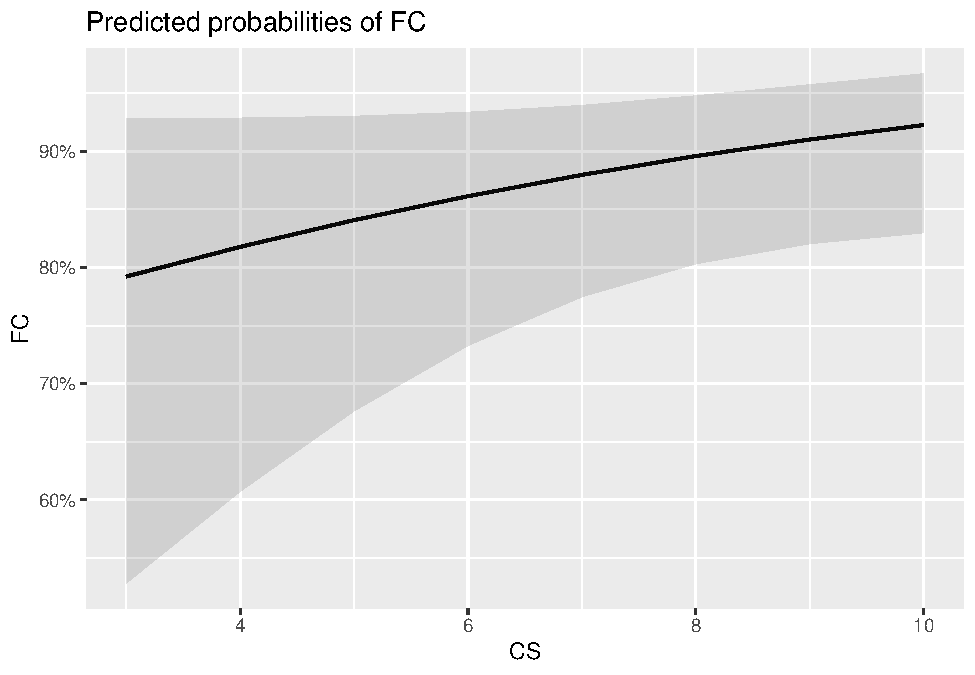
\includegraphics{model-funding-coveraeg-prediction_files/figure-latex/unnamed-chunk-6-1.pdf}

\begin{verbatim}
## 
## $H
\end{verbatim}

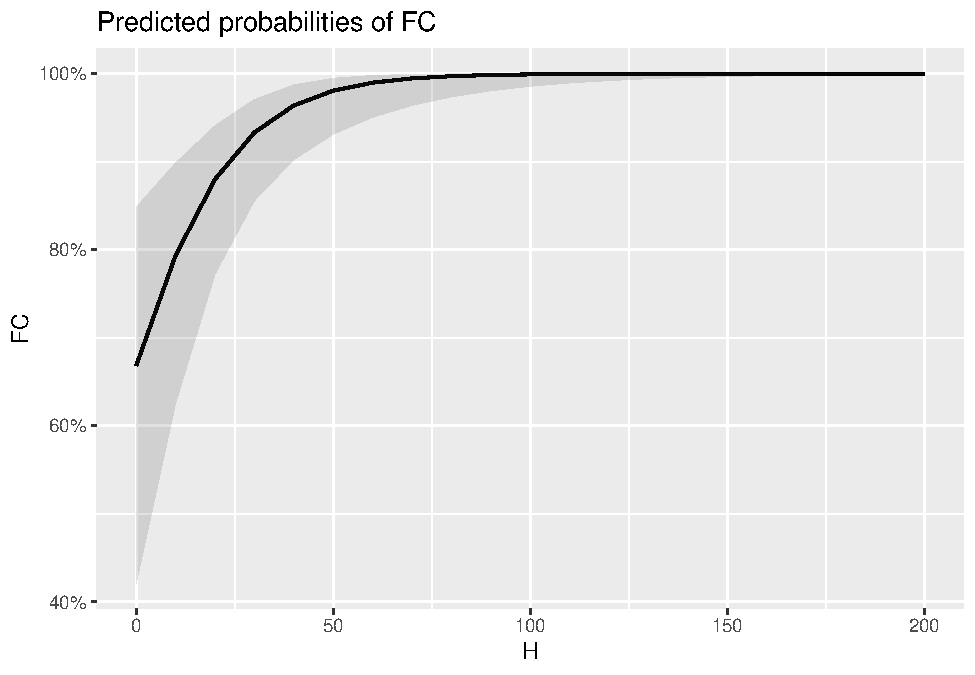
\includegraphics{model-funding-coveraeg-prediction_files/figure-latex/unnamed-chunk-6-2.pdf}

\begin{verbatim}
## 
## $TWR
\end{verbatim}

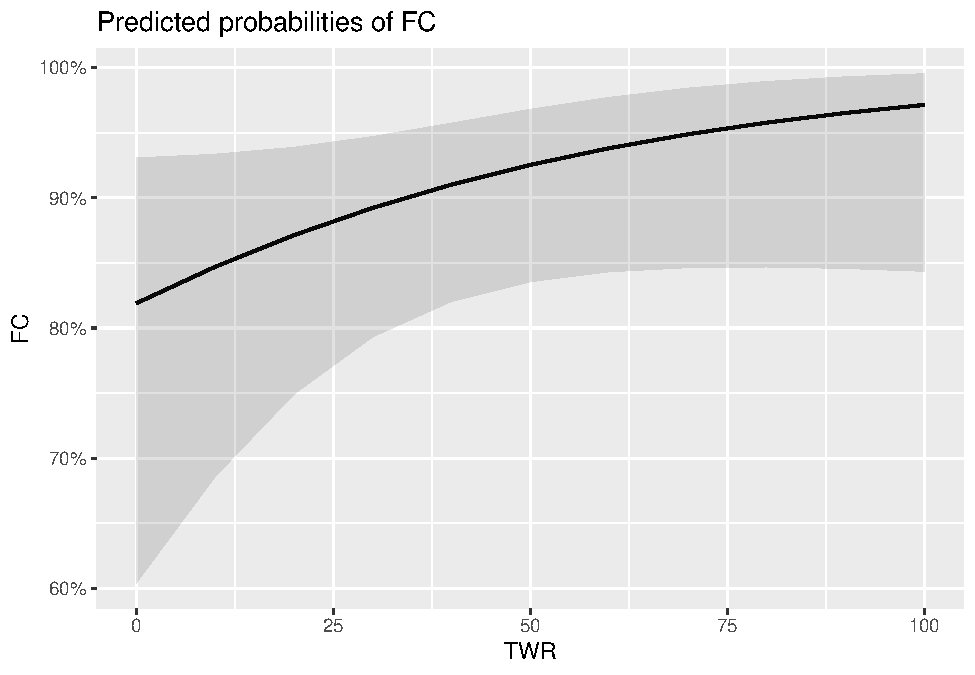
\includegraphics{model-funding-coveraeg-prediction_files/figure-latex/unnamed-chunk-6-3.pdf}

\begin{verbatim}
## 
## $NP
\end{verbatim}

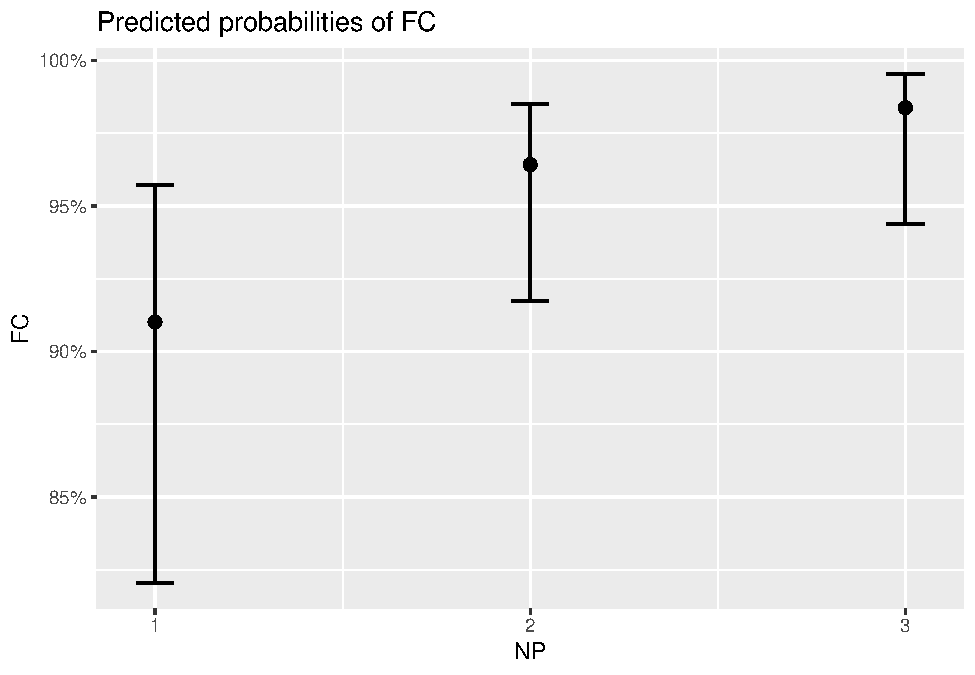
\includegraphics{model-funding-coveraeg-prediction_files/figure-latex/unnamed-chunk-6-4.pdf}

\begin{verbatim}
## 
## $TS
\end{verbatim}

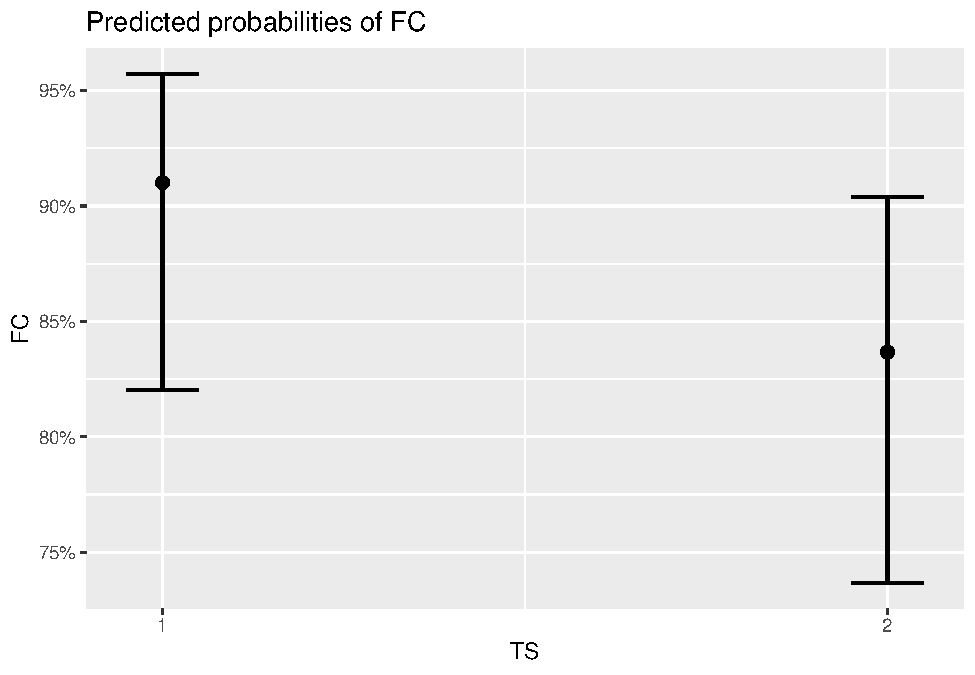
\includegraphics{model-funding-coveraeg-prediction_files/figure-latex/unnamed-chunk-6-5.pdf}

\newpage

\hypertarget{not_funded-1-25-vs-rest}{%
\subsection{Not\_funded + 1-25\% VS
Rest}\label{not_funded-1-25-vs-rest}}

\begin{verbatim}
##   x freq
## 1 1   36
## 2 2   54
## 3 3   46
## 4 4   74
## 5 5  102
## 6 6   91
\end{verbatim}

\begin{verbatim}
##   x freq
## 1 0   90
## 2 1  313
\end{verbatim}

\hypertarget{backward-elimination-model-1}{%
\subsection{Backward Elimination
Model}\label{backward-elimination-model-1}}

\begin{verbatim}
## 
## Call:
## glm(formula = FC ~ TA + E + OP + H + NP + FA + TS, family = "binomial", 
##     data = lm_DF)
## 
## Deviance Residuals: 
##     Min       1Q   Median       3Q      Max  
## -2.4301   0.1840   0.4926   0.7201   1.4204  
## 
## Coefficients:
##              Estimate Std. Error z value Pr(>|z|)    
## (Intercept)  2.383406   1.010389   2.359 0.018329 *  
## TA          -0.023932   0.013386  -1.788 0.073800 .  
## E           -0.110077   0.060819  -1.810 0.070312 .  
## OP          -0.115191   0.076896  -1.498 0.134132    
## H            0.033466   0.009783   3.421 0.000625 ***
## NP2          0.730882   0.293940   2.486 0.012901 *  
## NP3          1.428409   0.370387   3.857 0.000115 ***
## FA2          0.676051   0.382624   1.767 0.077248 .  
## FA3          1.964105   1.065483   1.843 0.065272 .  
## FA4          1.046163   0.777655   1.345 0.178535    
## FA5          1.213691   1.085638   1.118 0.263587    
## FA6         -0.031548   0.488857  -0.065 0.948544    
## TS2         -0.484149   0.272579  -1.776 0.075704 .  
## ---
## Signif. codes:  0 '***' 0.001 '**' 0.01 '*' 0.05 '.' 0.1 ' ' 1
## 
## (Dispersion parameter for binomial family taken to be 1)
## 
##     Null deviance: 428.05  on 402  degrees of freedom
## Residual deviance: 369.53  on 390  degrees of freedom
## AIC: 395.53
## 
## Number of Fisher Scoring iterations: 5
\end{verbatim}

\hypertarget{forward-selection}{%
\subsection{Forward selection}\label{forward-selection}}

\begin{verbatim}
## 
## Call:
## glm(formula = FC ~ H + NP + OP + FA + TS + E + TA, family = "binomial", 
##     data = lm_DF)
## 
## Deviance Residuals: 
##     Min       1Q   Median       3Q      Max  
## -2.4301   0.1840   0.4926   0.7201   1.4204  
## 
## Coefficients:
##              Estimate Std. Error z value Pr(>|z|)    
## (Intercept)  2.383406   1.010389   2.359 0.018329 *  
## H            0.033466   0.009783   3.421 0.000625 ***
## NP2          0.730882   0.293940   2.486 0.012901 *  
## NP3          1.428409   0.370387   3.857 0.000115 ***
## OP          -0.115191   0.076896  -1.498 0.134132    
## FA2          0.676051   0.382624   1.767 0.077248 .  
## FA3          1.964105   1.065483   1.843 0.065272 .  
## FA4          1.046163   0.777655   1.345 0.178535    
## FA5          1.213691   1.085638   1.118 0.263587    
## FA6         -0.031548   0.488857  -0.065 0.948544    
## TS2         -0.484149   0.272579  -1.776 0.075704 .  
## E           -0.110077   0.060819  -1.810 0.070312 .  
## TA          -0.023932   0.013386  -1.788 0.073800 .  
## ---
## Signif. codes:  0 '***' 0.001 '**' 0.01 '*' 0.05 '.' 0.1 ' ' 1
## 
## (Dispersion parameter for binomial family taken to be 1)
## 
##     Null deviance: 428.05  on 402  degrees of freedom
## Residual deviance: 369.53  on 390  degrees of freedom
## AIC: 395.53
## 
## Number of Fisher Scoring iterations: 5
\end{verbatim}

\hypertarget{stepwise}{%
\subsection{Stepwise}\label{stepwise}}

\begin{verbatim}
## 
## Call:
## glm(formula = FC ~ H + NP + OP + FA + TS + E + TA, family = "binomial", 
##     data = lm_DF)
## 
## Deviance Residuals: 
##     Min       1Q   Median       3Q      Max  
## -2.4301   0.1840   0.4926   0.7201   1.4204  
## 
## Coefficients:
##              Estimate Std. Error z value Pr(>|z|)    
## (Intercept)  2.383406   1.010389   2.359 0.018329 *  
## H            0.033466   0.009783   3.421 0.000625 ***
## NP2          0.730882   0.293940   2.486 0.012901 *  
## NP3          1.428409   0.370387   3.857 0.000115 ***
## OP          -0.115191   0.076896  -1.498 0.134132    
## FA2          0.676051   0.382624   1.767 0.077248 .  
## FA3          1.964105   1.065483   1.843 0.065272 .  
## FA4          1.046163   0.777655   1.345 0.178535    
## FA5          1.213691   1.085638   1.118 0.263587    
## FA6         -0.031548   0.488857  -0.065 0.948544    
## TS2         -0.484149   0.272579  -1.776 0.075704 .  
## E           -0.110077   0.060819  -1.810 0.070312 .  
## TA          -0.023932   0.013386  -1.788 0.073800 .  
## ---
## Signif. codes:  0 '***' 0.001 '**' 0.01 '*' 0.05 '.' 0.1 ' ' 1
## 
## (Dispersion parameter for binomial family taken to be 1)
## 
##     Null deviance: 428.05  on 402  degrees of freedom
## Residual deviance: 369.53  on 390  degrees of freedom
## AIC: 395.53
## 
## Number of Fisher Scoring iterations: 5
\end{verbatim}

\hypertarget{plots-1}{%
\subsection{Plots}\label{plots-1}}

\begin{verbatim}
## Data were 'prettified'. Consider using `terms="TA [all]"` to get smooth plots.
\end{verbatim}

\begin{verbatim}
## Data were 'prettified'. Consider using `terms="H [all]"` to get smooth plots.
\end{verbatim}

\begin{verbatim}
## $TA
\end{verbatim}

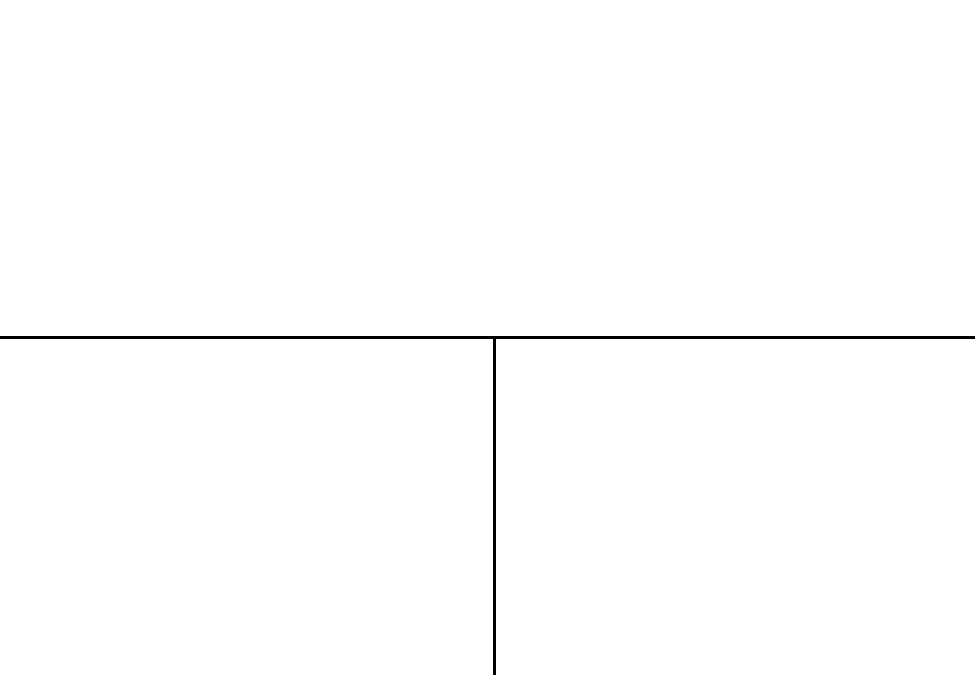
\includegraphics{model-funding-coveraeg-prediction_files/figure-latex/unnamed-chunk-11-1.pdf}

\begin{verbatim}
## 
## $E
\end{verbatim}

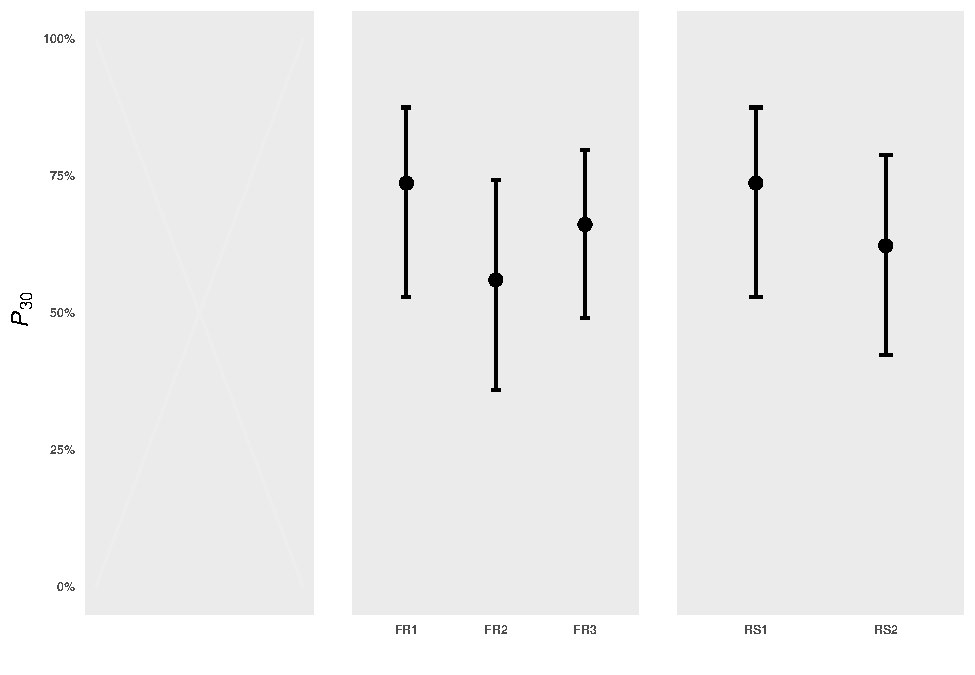
\includegraphics{model-funding-coveraeg-prediction_files/figure-latex/unnamed-chunk-11-2.pdf}

\begin{verbatim}
## 
## $OP
\end{verbatim}

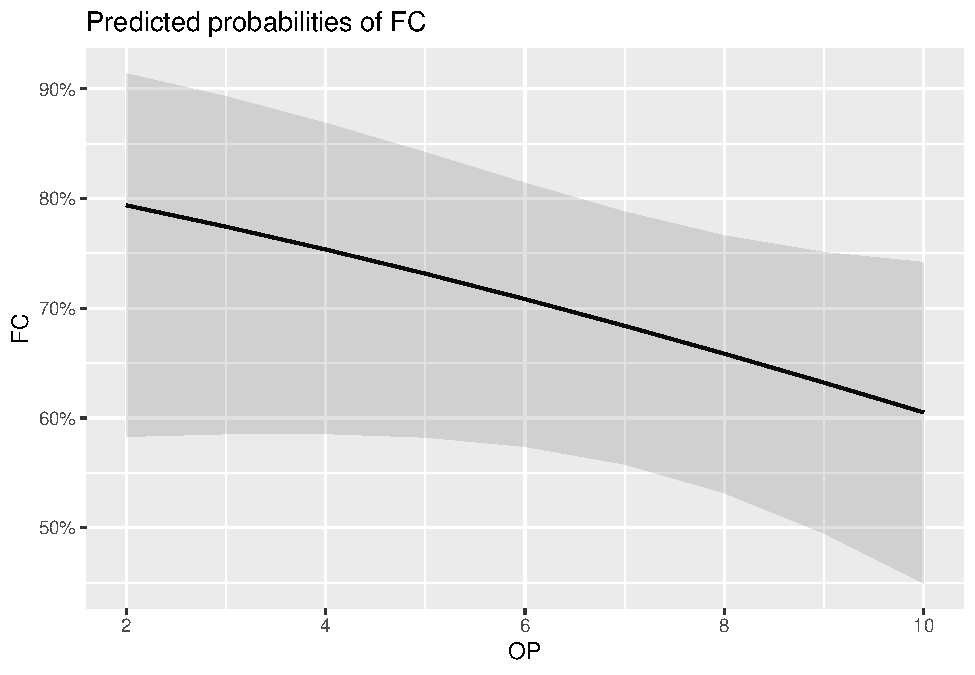
\includegraphics{model-funding-coveraeg-prediction_files/figure-latex/unnamed-chunk-11-3.pdf}

\begin{verbatim}
## 
## $H
\end{verbatim}

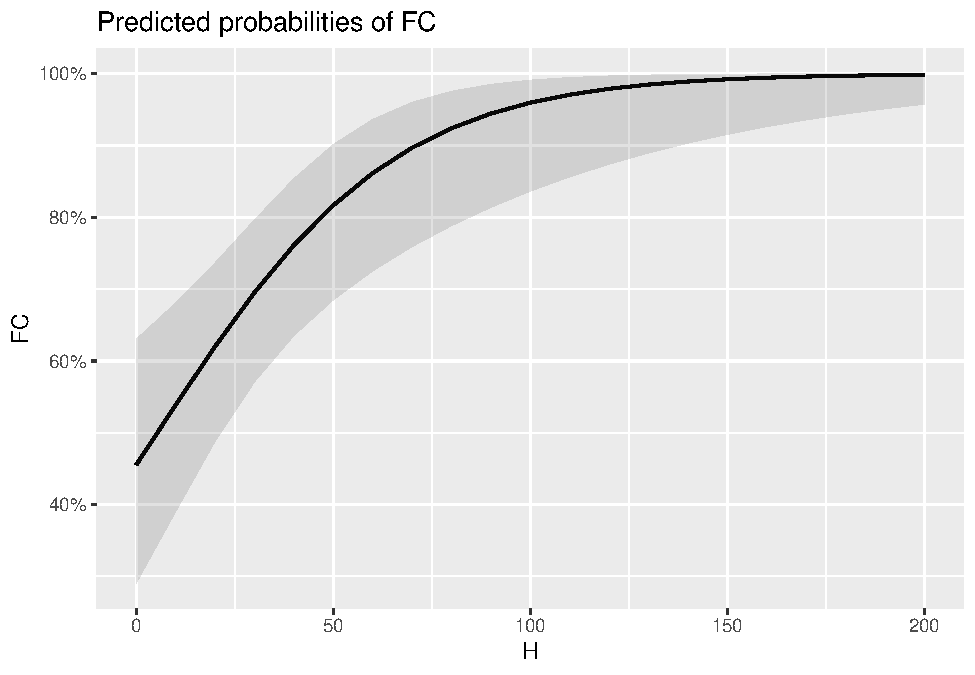
\includegraphics{model-funding-coveraeg-prediction_files/figure-latex/unnamed-chunk-11-4.pdf}

\begin{verbatim}
## 
## $NP
\end{verbatim}

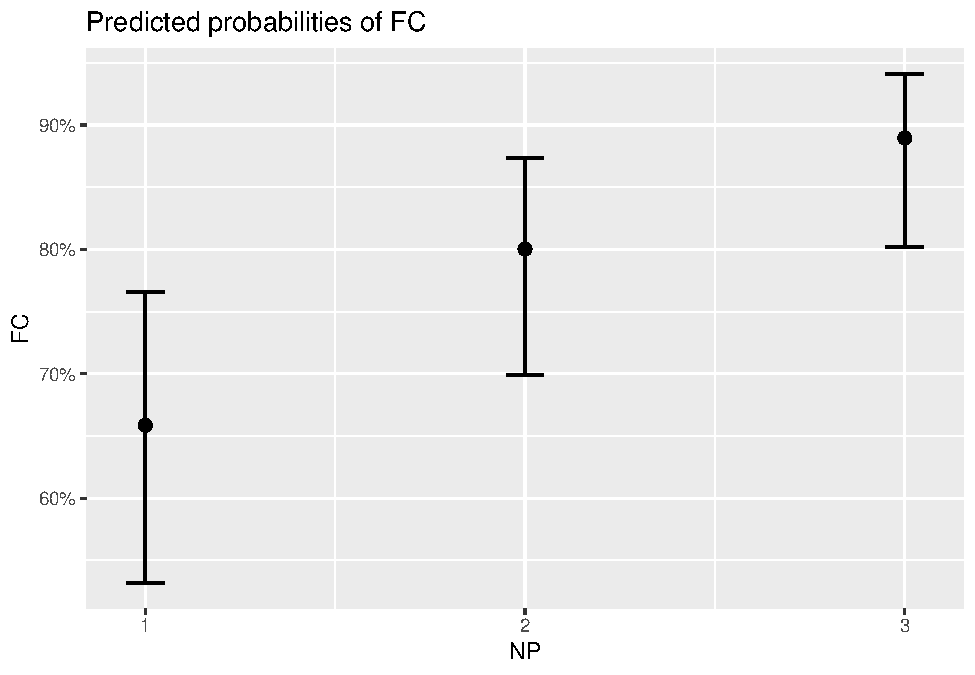
\includegraphics{model-funding-coveraeg-prediction_files/figure-latex/unnamed-chunk-11-5.pdf}

\begin{verbatim}
## 
## $FA
\end{verbatim}

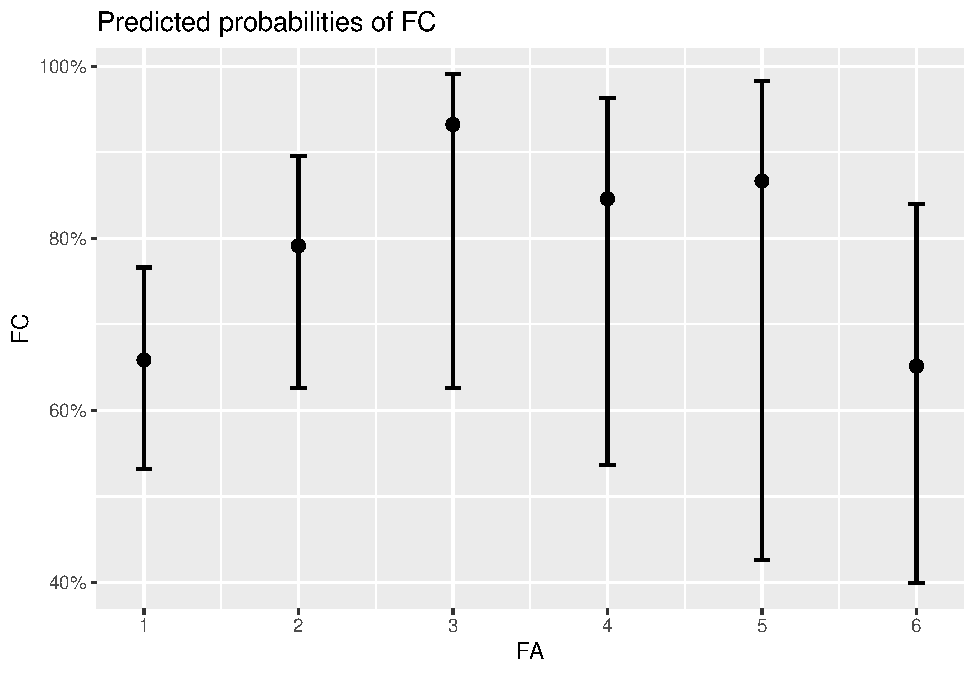
\includegraphics{model-funding-coveraeg-prediction_files/figure-latex/unnamed-chunk-11-6.pdf}

\begin{verbatim}
## 
## $TS
\end{verbatim}

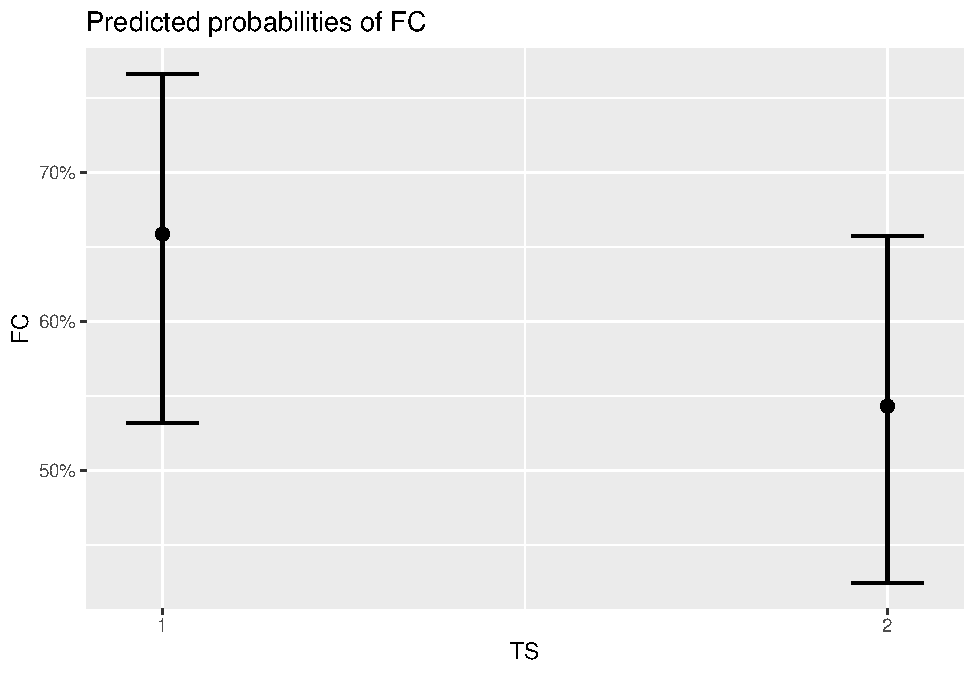
\includegraphics{model-funding-coveraeg-prediction_files/figure-latex/unnamed-chunk-11-7.pdf}

\newpage

\hypertarget{not_funded1-25-50-vs-rest}{%
\subsection{Not\_funded+1-25\%-50\% VS
Rest}\label{not_funded1-25-50-vs-rest}}

\begin{verbatim}
##   x freq
## 1 1   36
## 2 2   54
## 3 3   46
## 4 4   74
## 5 5  102
## 6 6   91
\end{verbatim}

\begin{verbatim}
##   x freq
## 1 0  136
## 2 1  267
\end{verbatim}

\hypertarget{backward-elimination-model-2}{%
\subsection{Backward Elimination
Model}\label{backward-elimination-model-2}}

\begin{verbatim}
## 
## Call:
## glm(formula = FC ~ NASA + TA + E + Task + H + TWR + NP + FA, 
##     family = "binomial", data = lm_DF)
## 
## Deviance Residuals: 
##     Min       1Q   Median       3Q      Max  
## -2.0760  -1.0893   0.5542   0.8836   1.6093  
## 
## Coefficients:
##              Estimate Std. Error z value Pr(>|z|)    
## (Intercept)  1.401966   1.330792   1.053  0.29212    
## NASA         0.038822   0.021803   1.781  0.07498 .  
## TA          -0.025466   0.013239  -1.924  0.05441 .  
## E           -0.173462   0.054195  -3.201  0.00137 ** 
## Task        -0.052055   0.032407  -1.606  0.10821    
## H            0.024580   0.007649   3.213  0.00131 ** 
## TWR          0.016066   0.007639   2.103  0.03546 *  
## NP2          0.530421   0.266103   1.993  0.04623 *  
## NP3          1.114839   0.321738   3.465  0.00053 ***
## FA2          0.241171   0.314788   0.766  0.44359    
## FA3          1.247971   0.672595   1.855  0.06353 .  
## FA4          1.386376   0.659090   2.103  0.03542 *  
## FA5          1.764003   1.073278   1.644  0.10027    
## FA6          0.238172   0.463196   0.514  0.60712    
## ---
## Signif. codes:  0 '***' 0.001 '**' 0.01 '*' 0.05 '.' 0.1 ' ' 1
## 
## (Dispersion parameter for binomial family taken to be 1)
## 
##     Null deviance: 515.31  on 402  degrees of freedom
## Residual deviance: 449.71  on 389  degrees of freedom
## AIC: 477.71
## 
## Number of Fisher Scoring iterations: 4
\end{verbatim}

\hypertarget{forward-selection-model-1}{%
\subsection{Forward selection model}\label{forward-selection-model-1}}

\begin{verbatim}
## 
## Call:
## glm(formula = FC ~ H + NP + E + FA + TWR + OP, family = "binomial", 
##     data = lm_DF)
## 
## Deviance Residuals: 
##     Min       1Q   Median       3Q      Max  
## -2.1485  -1.0602   0.5408   0.8989   1.6680  
## 
## Coefficients:
##              Estimate Std. Error z value Pr(>|z|)    
## (Intercept)  0.292271   0.702334   0.416 0.677305    
## H            0.024436   0.007460   3.276 0.001055 ** 
## NP2          0.514244   0.263893   1.949 0.051334 .  
## NP3          1.105446   0.314243   3.518 0.000435 ***
## E           -0.146719   0.052623  -2.788 0.005301 ** 
## FA2          0.299181   0.309449   0.967 0.333634    
## FA3          1.203438   0.670516   1.795 0.072687 .  
## FA4          1.326457   0.656301   2.021 0.043268 *  
## FA5          1.902042   1.075300   1.769 0.076919 .  
## FA6          0.145160   0.458522   0.317 0.751561    
## TWR          0.017144   0.007577   2.263 0.023650 *  
## OP          -0.102437   0.066409  -1.543 0.122944    
## ---
## Signif. codes:  0 '***' 0.001 '**' 0.01 '*' 0.05 '.' 0.1 ' ' 1
## 
## (Dispersion parameter for binomial family taken to be 1)
## 
##     Null deviance: 515.31  on 402  degrees of freedom
## Residual deviance: 453.57  on 391  degrees of freedom
## AIC: 477.57
## 
## Number of Fisher Scoring iterations: 4
\end{verbatim}

\hypertarget{stepwise-model-1}{%
\subsection{Stepwise model}\label{stepwise-model-1}}

\begin{verbatim}
## 
## Call:
## glm(formula = FC ~ H + NP + E + FA + TWR + OP, family = "binomial", 
##     data = lm_DF)
## 
## Deviance Residuals: 
##     Min       1Q   Median       3Q      Max  
## -2.1485  -1.0602   0.5408   0.8989   1.6680  
## 
## Coefficients:
##              Estimate Std. Error z value Pr(>|z|)    
## (Intercept)  0.292271   0.702334   0.416 0.677305    
## H            0.024436   0.007460   3.276 0.001055 ** 
## NP2          0.514244   0.263893   1.949 0.051334 .  
## NP3          1.105446   0.314243   3.518 0.000435 ***
## E           -0.146719   0.052623  -2.788 0.005301 ** 
## FA2          0.299181   0.309449   0.967 0.333634    
## FA3          1.203438   0.670516   1.795 0.072687 .  
## FA4          1.326457   0.656301   2.021 0.043268 *  
## FA5          1.902042   1.075300   1.769 0.076919 .  
## FA6          0.145160   0.458522   0.317 0.751561    
## TWR          0.017144   0.007577   2.263 0.023650 *  
## OP          -0.102437   0.066409  -1.543 0.122944    
## ---
## Signif. codes:  0 '***' 0.001 '**' 0.01 '*' 0.05 '.' 0.1 ' ' 1
## 
## (Dispersion parameter for binomial family taken to be 1)
## 
##     Null deviance: 515.31  on 402  degrees of freedom
## Residual deviance: 453.57  on 391  degrees of freedom
## AIC: 477.57
## 
## Number of Fisher Scoring iterations: 4
\end{verbatim}

\hypertarget{plots-2}{%
\subsection{Plots}\label{plots-2}}

\begin{verbatim}
## Data were 'prettified'. Consider using `terms="NASA [all]"` to get smooth plots.
\end{verbatim}

\begin{verbatim}
## Data were 'prettified'. Consider using `terms="TA [all]"` to get smooth plots.
\end{verbatim}

\begin{verbatim}
## Data were 'prettified'. Consider using `terms="Task [all]"` to get smooth plots.
\end{verbatim}

\begin{verbatim}
## Data were 'prettified'. Consider using `terms="H [all]"` to get smooth plots.
\end{verbatim}

\begin{verbatim}
## $NASA
\end{verbatim}

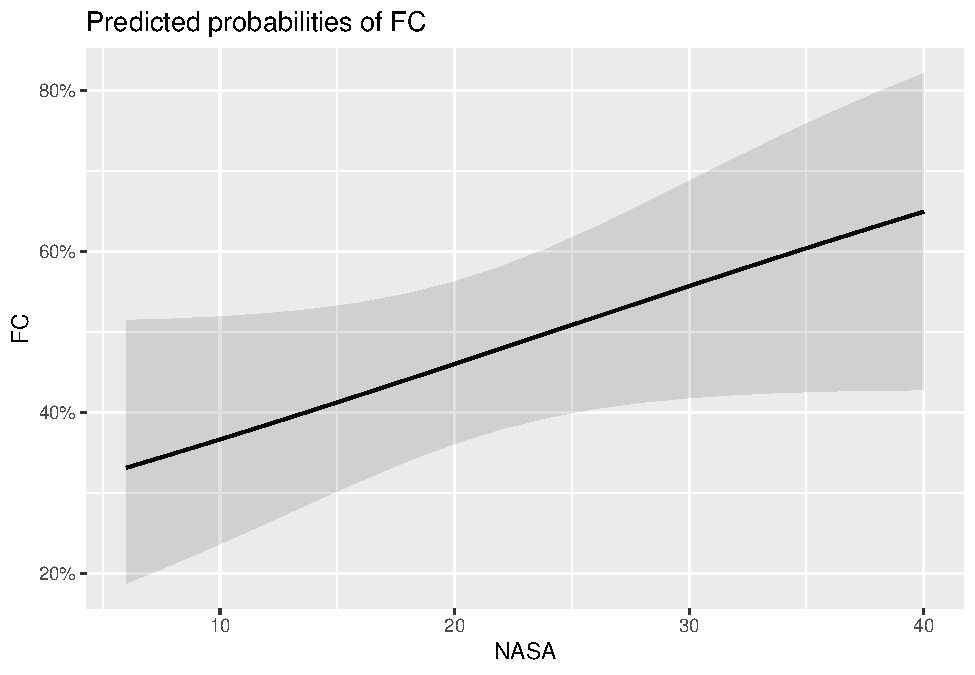
\includegraphics{model-funding-coveraeg-prediction_files/figure-latex/unnamed-chunk-16-1.pdf}

\begin{verbatim}
## 
## $TA
\end{verbatim}

\includegraphics{model-funding-coveraeg-prediction_files/figure-latex/unnamed-chunk-16-2.pdf}

\begin{verbatim}
## 
## $E
\end{verbatim}

\includegraphics{model-funding-coveraeg-prediction_files/figure-latex/unnamed-chunk-16-3.pdf}

\begin{verbatim}
## 
## $Task
\end{verbatim}

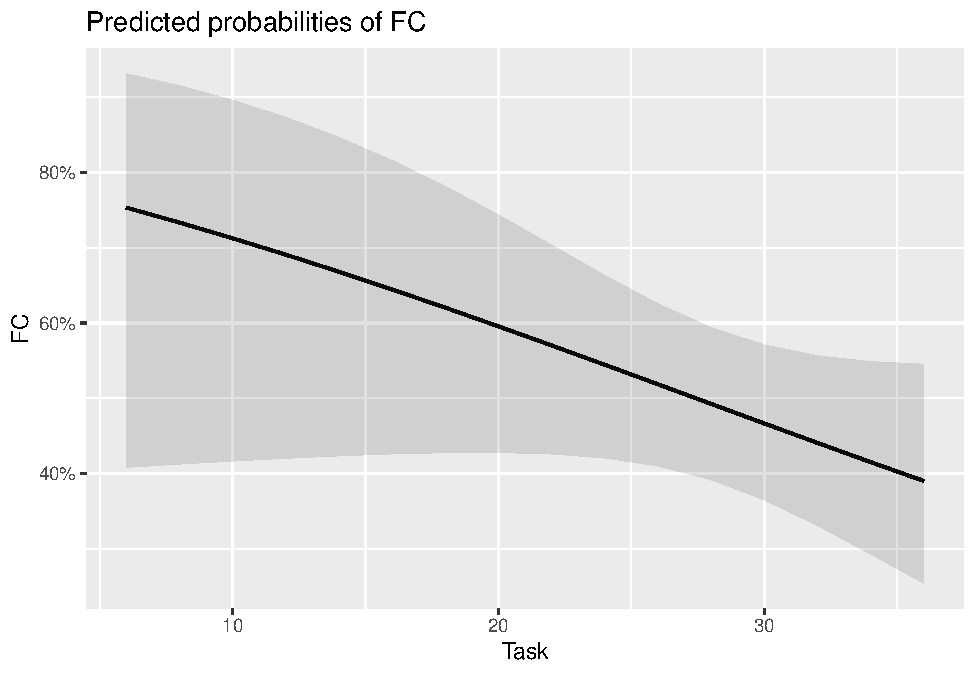
\includegraphics{model-funding-coveraeg-prediction_files/figure-latex/unnamed-chunk-16-4.pdf}

\begin{verbatim}
## 
## $H
\end{verbatim}

\includegraphics{model-funding-coveraeg-prediction_files/figure-latex/unnamed-chunk-16-5.pdf}

\begin{verbatim}
## 
## $TWR
\end{verbatim}

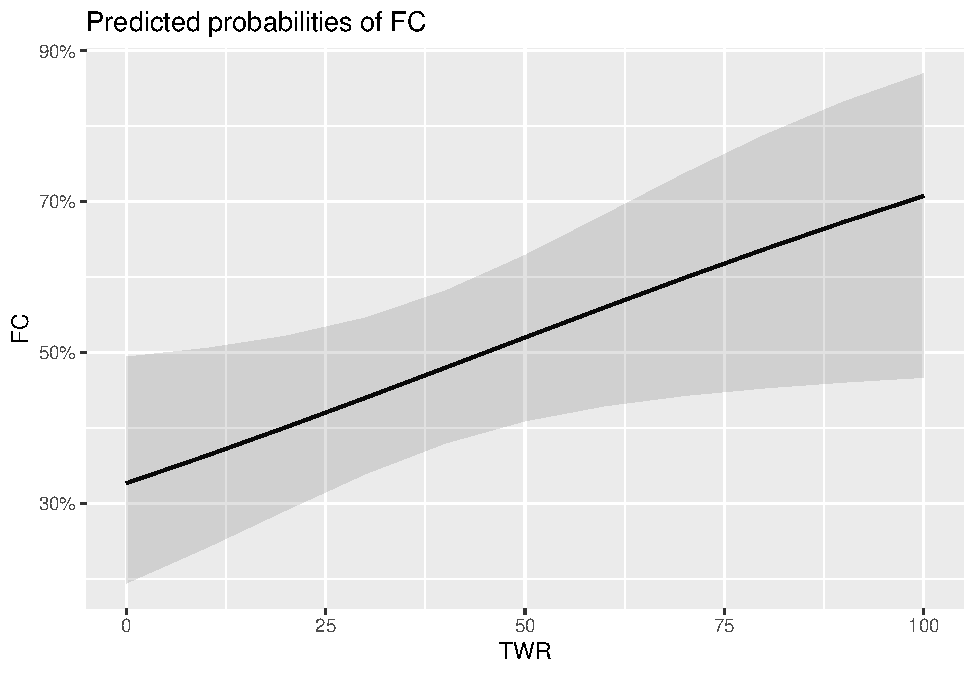
\includegraphics{model-funding-coveraeg-prediction_files/figure-latex/unnamed-chunk-16-6.pdf}

\begin{verbatim}
## 
## $NP
\end{verbatim}

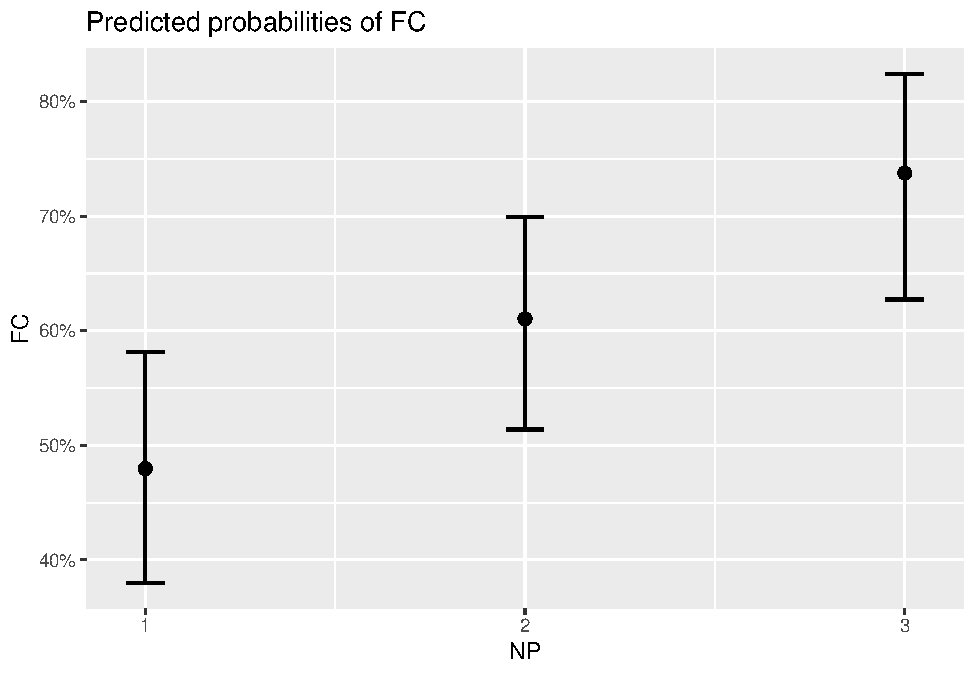
\includegraphics{model-funding-coveraeg-prediction_files/figure-latex/unnamed-chunk-16-7.pdf}

\begin{verbatim}
## 
## $FA
\end{verbatim}

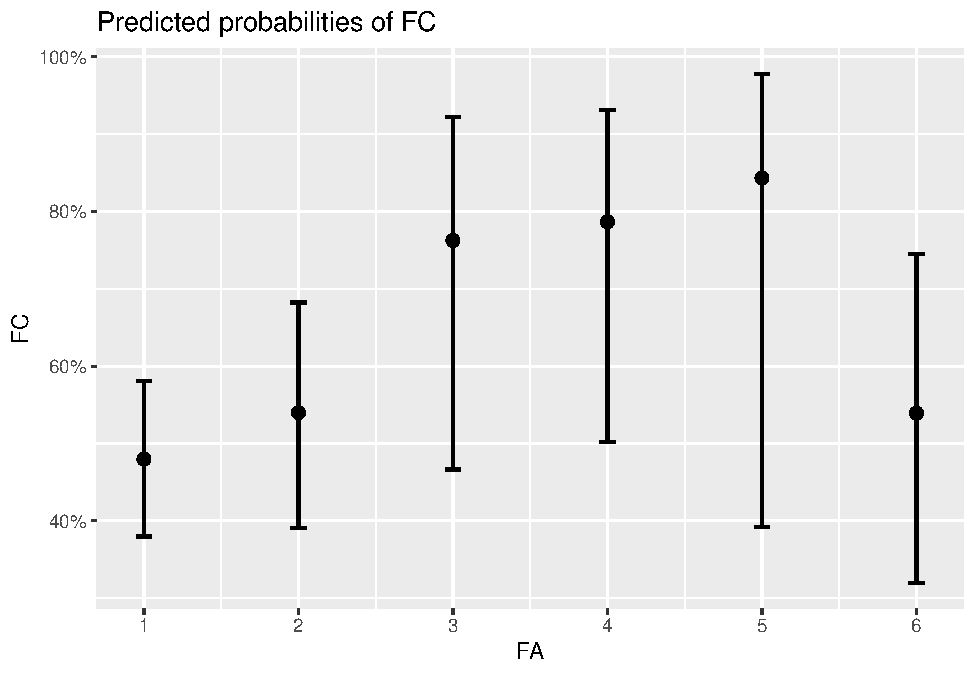
\includegraphics{model-funding-coveraeg-prediction_files/figure-latex/unnamed-chunk-16-8.pdf}

\newpage

\hypertarget{not_funded1-25-50-75-vs-rest}{%
\subsection{Not\_funded+1-25\%-50-75\% VS
Rest}\label{not_funded1-25-50-75-vs-rest}}

\begin{verbatim}
##   x freq
## 1 1   36
## 2 2   54
## 3 3   46
## 4 4   74
## 5 5  102
## 6 6   91
\end{verbatim}

\begin{verbatim}
##   x freq
## 1 0  210
## 2 1  193
\end{verbatim}

\hypertarget{backward-elimination-model-3}{%
\subsection{Backward Elimination
Model}\label{backward-elimination-model-3}}

\begin{verbatim}
## 
## Call:
## glm(formula = FC ~ TA + E + OP + H + RS + TWR + FA + TS, family = "binomial", 
##     data = lm_DF)
## 
## Deviance Residuals: 
##     Min       1Q   Median       3Q      Max  
## -1.9735  -1.0145  -0.6707   1.1196   1.9882  
## 
## Coefficients:
##              Estimate Std. Error z value Pr(>|z|)   
## (Intercept)  1.190248   0.847673   1.404  0.16028   
## TA          -0.016566   0.011046  -1.500  0.13368   
## E           -0.098280   0.049702  -1.977  0.04800 * 
## OP          -0.108308   0.061463  -1.762  0.07804 . 
## H            0.010820   0.005573   1.942  0.05219 . 
## RS2         -0.436695   0.220332  -1.982  0.04748 * 
## TWR          0.021334   0.006960   3.065  0.00217 **
## FA2         -0.066633   0.287263  -0.232  0.81657   
## FA3          1.643709   0.609770   2.696  0.00703 **
## FA4          1.442779   0.542853   2.658  0.00787 **
## FA5          0.800573   0.656070   1.220  0.22237   
## FA6         -0.032084   0.442106  -0.073  0.94215   
## TS2         -0.543443   0.221893  -2.449  0.01432 * 
## ---
## Signif. codes:  0 '***' 0.001 '**' 0.01 '*' 0.05 '.' 0.1 ' ' 1
## 
## (Dispersion parameter for binomial family taken to be 1)
## 
##     Null deviance: 557.96  on 402  degrees of freedom
## Residual deviance: 504.29  on 390  degrees of freedom
## AIC: 530.29
## 
## Number of Fisher Scoring iterations: 4
\end{verbatim}

\hypertarget{forward-selection-1}{%
\subsection{Forward selection}\label{forward-selection-1}}

\begin{verbatim}
## 
## Call:
## glm(formula = FC ~ FA + TWR + H + TS + RS + OP + E + TA, family = "binomial", 
##     data = lm_DF)
## 
## Deviance Residuals: 
##     Min       1Q   Median       3Q      Max  
## -1.9735  -1.0145  -0.6707   1.1196   1.9882  
## 
## Coefficients:
##              Estimate Std. Error z value Pr(>|z|)   
## (Intercept)  1.190248   0.847673   1.404  0.16028   
## FA2         -0.066633   0.287263  -0.232  0.81657   
## FA3          1.643709   0.609770   2.696  0.00703 **
## FA4          1.442779   0.542853   2.658  0.00787 **
## FA5          0.800573   0.656070   1.220  0.22237   
## FA6         -0.032084   0.442106  -0.073  0.94215   
## TWR          0.021334   0.006960   3.065  0.00217 **
## H            0.010820   0.005573   1.942  0.05219 . 
## TS2         -0.543443   0.221893  -2.449  0.01432 * 
## RS2         -0.436695   0.220332  -1.982  0.04748 * 
## OP          -0.108308   0.061463  -1.762  0.07804 . 
## E           -0.098280   0.049702  -1.977  0.04800 * 
## TA          -0.016566   0.011046  -1.500  0.13368   
## ---
## Signif. codes:  0 '***' 0.001 '**' 0.01 '*' 0.05 '.' 0.1 ' ' 1
## 
## (Dispersion parameter for binomial family taken to be 1)
## 
##     Null deviance: 557.96  on 402  degrees of freedom
## Residual deviance: 504.29  on 390  degrees of freedom
## AIC: 530.29
## 
## Number of Fisher Scoring iterations: 4
\end{verbatim}

\hypertarget{stepwise-1}{%
\subsection{Stepwise}\label{stepwise-1}}

\begin{verbatim}
## 
## Call:
## glm(formula = FC ~ FA + TWR + H + TS + RS + OP + E + TA, family = "binomial", 
##     data = lm_DF)
## 
## Deviance Residuals: 
##     Min       1Q   Median       3Q      Max  
## -1.9735  -1.0145  -0.6707   1.1196   1.9882  
## 
## Coefficients:
##              Estimate Std. Error z value Pr(>|z|)   
## (Intercept)  1.190248   0.847673   1.404  0.16028   
## FA2         -0.066633   0.287263  -0.232  0.81657   
## FA3          1.643709   0.609770   2.696  0.00703 **
## FA4          1.442779   0.542853   2.658  0.00787 **
## FA5          0.800573   0.656070   1.220  0.22237   
## FA6         -0.032084   0.442106  -0.073  0.94215   
## TWR          0.021334   0.006960   3.065  0.00217 **
## H            0.010820   0.005573   1.942  0.05219 . 
## TS2         -0.543443   0.221893  -2.449  0.01432 * 
## RS2         -0.436695   0.220332  -1.982  0.04748 * 
## OP          -0.108308   0.061463  -1.762  0.07804 . 
## E           -0.098280   0.049702  -1.977  0.04800 * 
## TA          -0.016566   0.011046  -1.500  0.13368   
## ---
## Signif. codes:  0 '***' 0.001 '**' 0.01 '*' 0.05 '.' 0.1 ' ' 1
## 
## (Dispersion parameter for binomial family taken to be 1)
## 
##     Null deviance: 557.96  on 402  degrees of freedom
## Residual deviance: 504.29  on 390  degrees of freedom
## AIC: 530.29
## 
## Number of Fisher Scoring iterations: 4
\end{verbatim}

\hypertarget{plots-3}{%
\subsection{Plots}\label{plots-3}}

\begin{verbatim}
## Data were 'prettified'. Consider using `terms="TA [all]"` to get smooth plots.
\end{verbatim}

\begin{verbatim}
## Data were 'prettified'. Consider using `terms="H [all]"` to get smooth plots.
\end{verbatim}

\begin{verbatim}
## $TA
\end{verbatim}

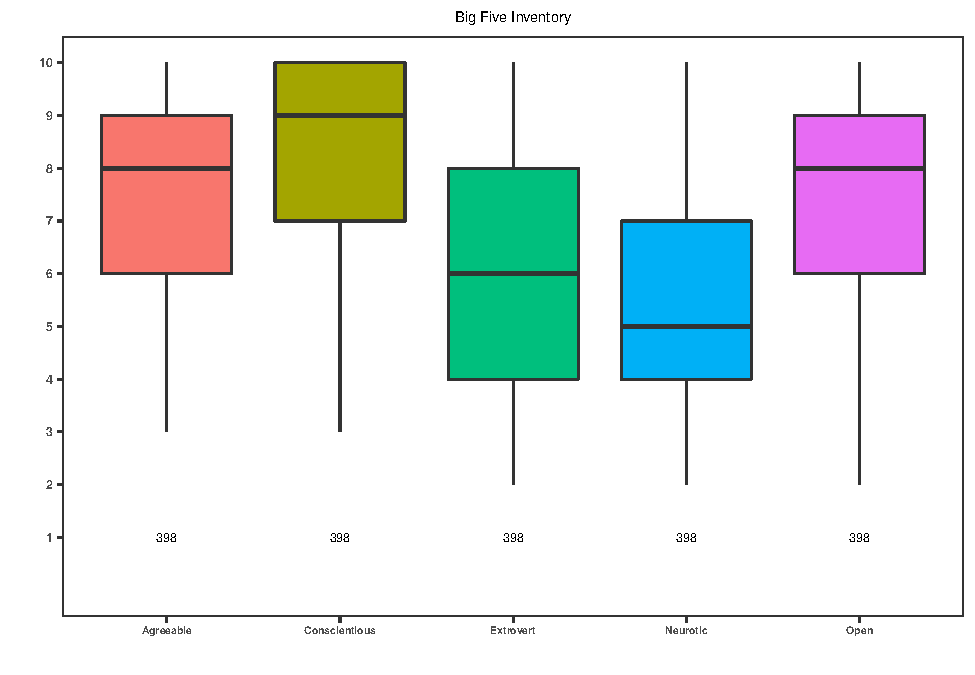
\includegraphics{model-funding-coveraeg-prediction_files/figure-latex/unnamed-chunk-21-1.pdf}

\begin{verbatim}
## 
## $E
\end{verbatim}

\includegraphics{model-funding-coveraeg-prediction_files/figure-latex/unnamed-chunk-21-2.pdf}

\begin{verbatim}
## 
## $OP
\end{verbatim}

\includegraphics{model-funding-coveraeg-prediction_files/figure-latex/unnamed-chunk-21-3.pdf}

\begin{verbatim}
## 
## $H
\end{verbatim}

\includegraphics{model-funding-coveraeg-prediction_files/figure-latex/unnamed-chunk-21-4.pdf}

\begin{verbatim}
## 
## $RS
\end{verbatim}

\includegraphics{model-funding-coveraeg-prediction_files/figure-latex/unnamed-chunk-21-5.pdf}

\begin{verbatim}
## 
## $TWR
\end{verbatim}

\includegraphics{model-funding-coveraeg-prediction_files/figure-latex/unnamed-chunk-21-6.pdf}

\begin{verbatim}
## 
## $FA
\end{verbatim}

\includegraphics{model-funding-coveraeg-prediction_files/figure-latex/unnamed-chunk-21-7.pdf}

\begin{verbatim}
## 
## $TS
\end{verbatim}

\includegraphics{model-funding-coveraeg-prediction_files/figure-latex/unnamed-chunk-21-8.pdf}

\newpage

\hypertarget{full-funded-vs-rest}{%
\subsection{Full funded VS Rest}\label{full-funded-vs-rest}}

\begin{verbatim}
##   x freq
## 1 1   36
## 2 2   54
## 3 3   46
## 4 4   74
## 5 5  102
## 6 6   91
\end{verbatim}

\begin{verbatim}
##   x freq
## 1 0  312
## 2 1   91
\end{verbatim}

\hypertarget{backward-elimination-model-4}{%
\subsection{Backward Elimination
Model}\label{backward-elimination-model-4}}

\begin{verbatim}
## 
## Call:
## glm(formula = FC ~ OP + Task + RS + TWR + FA + TS, family = "binomial", 
##     data = lm_DF)
## 
## Deviance Residuals: 
##     Min       1Q   Median       3Q      Max  
## -1.5430  -0.7173  -0.5335  -0.3289   2.4630  
## 
## Coefficients:
##             Estimate Std. Error z value Pr(>|z|)    
## (Intercept) -3.47358    1.15175  -3.016  0.00256 ** 
## OP          -0.15429    0.07389  -2.088  0.03679 *  
## Task         0.06333    0.03487   1.816  0.06933 .  
## RS2         -0.41016    0.25833  -1.588  0.11234    
## TWR          0.03949    0.00851   4.640 3.48e-06 ***
## FA2          0.17613    0.34403   0.512  0.60868    
## FA3          0.98777    0.51908   1.903  0.05705 .  
## FA4          1.62151    0.49447   3.279  0.00104 ** 
## FA5          0.42263    0.82670   0.511  0.60919    
## FA6          0.52294    0.52196   1.002  0.31640    
## TS2         -0.38176    0.26261  -1.454  0.14603    
## ---
## Signif. codes:  0 '***' 0.001 '**' 0.01 '*' 0.05 '.' 0.1 ' ' 1
## 
## (Dispersion parameter for binomial family taken to be 1)
## 
##     Null deviance: 430.53  on 402  degrees of freedom
## Residual deviance: 382.88  on 392  degrees of freedom
## AIC: 404.88
## 
## Number of Fisher Scoring iterations: 4
\end{verbatim}

\hypertarget{forward-selection-2}{%
\subsection{Forward selection}\label{forward-selection-2}}

\begin{verbatim}
## 
## Call:
## glm(formula = FC ~ TWR + FA + OP + Task + RS + TS, family = "binomial", 
##     data = lm_DF)
## 
## Deviance Residuals: 
##     Min       1Q   Median       3Q      Max  
## -1.5430  -0.7173  -0.5335  -0.3289   2.4630  
## 
## Coefficients:
##             Estimate Std. Error z value Pr(>|z|)    
## (Intercept) -3.47358    1.15175  -3.016  0.00256 ** 
## TWR          0.03949    0.00851   4.640 3.48e-06 ***
## FA2          0.17613    0.34403   0.512  0.60868    
## FA3          0.98777    0.51908   1.903  0.05705 .  
## FA4          1.62151    0.49447   3.279  0.00104 ** 
## FA5          0.42263    0.82670   0.511  0.60919    
## FA6          0.52294    0.52196   1.002  0.31640    
## OP          -0.15429    0.07389  -2.088  0.03679 *  
## Task         0.06333    0.03487   1.816  0.06933 .  
## RS2         -0.41016    0.25833  -1.588  0.11234    
## TS2         -0.38176    0.26261  -1.454  0.14603    
## ---
## Signif. codes:  0 '***' 0.001 '**' 0.01 '*' 0.05 '.' 0.1 ' ' 1
## 
## (Dispersion parameter for binomial family taken to be 1)
## 
##     Null deviance: 430.53  on 402  degrees of freedom
## Residual deviance: 382.88  on 392  degrees of freedom
## AIC: 404.88
## 
## Number of Fisher Scoring iterations: 4
\end{verbatim}

\hypertarget{stepwise-2}{%
\subsection{Stepwise}\label{stepwise-2}}

\begin{verbatim}
## 
## Call:
## glm(formula = FC ~ TWR + FA + OP + Task + RS + TS, family = "binomial", 
##     data = lm_DF)
## 
## Deviance Residuals: 
##     Min       1Q   Median       3Q      Max  
## -1.5430  -0.7173  -0.5335  -0.3289   2.4630  
## 
## Coefficients:
##             Estimate Std. Error z value Pr(>|z|)    
## (Intercept) -3.47358    1.15175  -3.016  0.00256 ** 
## TWR          0.03949    0.00851   4.640 3.48e-06 ***
## FA2          0.17613    0.34403   0.512  0.60868    
## FA3          0.98777    0.51908   1.903  0.05705 .  
## FA4          1.62151    0.49447   3.279  0.00104 ** 
## FA5          0.42263    0.82670   0.511  0.60919    
## FA6          0.52294    0.52196   1.002  0.31640    
## OP          -0.15429    0.07389  -2.088  0.03679 *  
## Task         0.06333    0.03487   1.816  0.06933 .  
## RS2         -0.41016    0.25833  -1.588  0.11234    
## TS2         -0.38176    0.26261  -1.454  0.14603    
## ---
## Signif. codes:  0 '***' 0.001 '**' 0.01 '*' 0.05 '.' 0.1 ' ' 1
## 
## (Dispersion parameter for binomial family taken to be 1)
## 
##     Null deviance: 430.53  on 402  degrees of freedom
## Residual deviance: 382.88  on 392  degrees of freedom
## AIC: 404.88
## 
## Number of Fisher Scoring iterations: 4
\end{verbatim}

\hypertarget{plots-4}{%
\subsection{Plots}\label{plots-4}}

\begin{verbatim}
## Data were 'prettified'. Consider using `terms="Task [all]"` to get smooth plots.
\end{verbatim}

\begin{verbatim}
## $OP
\end{verbatim}

\includegraphics{model-funding-coveraeg-prediction_files/figure-latex/unnamed-chunk-26-1.pdf}

\begin{verbatim}
## 
## $Task
\end{verbatim}

\includegraphics{model-funding-coveraeg-prediction_files/figure-latex/unnamed-chunk-26-2.pdf}

\begin{verbatim}
## 
## $RS
\end{verbatim}

\includegraphics{model-funding-coveraeg-prediction_files/figure-latex/unnamed-chunk-26-3.pdf}

\begin{verbatim}
## 
## $TWR
\end{verbatim}

\includegraphics{model-funding-coveraeg-prediction_files/figure-latex/unnamed-chunk-26-4.pdf}

\begin{verbatim}
## 
## $FA
\end{verbatim}

\includegraphics{model-funding-coveraeg-prediction_files/figure-latex/unnamed-chunk-26-5.pdf}

\begin{verbatim}
## 
## $TS
\end{verbatim}

\includegraphics{model-funding-coveraeg-prediction_files/figure-latex/unnamed-chunk-26-6.pdf}


\end{document}
